

\part{Getting started}
\label{part:GettingStarted}

\chapter{Overview}

\section{Introduction}

This part of the book will run the reader through the LedgerSMB using an example
startup company run by Jack: Example Inc, which starts its life as a computer parts
store for the business to business market.

Jack just completed incorporation of Example and is ready to start doing business.
Before starting his operation Jack decides to look for tooling to run his operation
efficiently.

The other chapters in this part of the book show you what steps Jack has to go through
to get LedgerSMB up and running for Example, as well as the steps he has to take to
keep LedgerSMB in good health.

Due to its success Example will grow, posing new challenges to LedgerSMB and we'll show
you how Jack can change the configuration to adapt to his growing business's needs.

Jack chooses to use a hosted LedgerSMB, so he doesn't need to concern himself with the
technical details of getting the application up and running. Instead he can start by setting
up the company database immediately.

In \charef{cha:CompanyCreation} and \charef{cha:the-first-login} Jack goes through the
steps of setting up a basic company. The chapters after that may not apply to every
business. \charef{cha:building-up-stock}, \charef{cha:ramping-up-to-the-first-sale} and
\charef{cha:shipping-sales} apply to businesses dealing with physical goods: buying,
selling and shipping. \charef{cha:invoicing} discusses how to handle invoicing from LedgerSMB.
\charef{cha:customer-payments}, \charef{cha:vendor-payments} and \charef{cha:monitoring-arrears}
discuss how to manage accounts receivable and payable including arrears monitoring.

@@@ more chapters??

\section{LedgerSMB, because...}

Jack finds several tools which suit his requirements to some extent or another.
After evaluation of his options he decides to use LedgerSMB for the following reasons:

\begin{itemize}
\item Centralized data storage
\item Actively developed
\item Development team with security focus
\item Access to the application requires only a web browser
\item Integrated sales, shipping, invoicing, purchasing and accounting
\item Open source solution, so no vendor lock in
\item The roadmap appeals to him, because it has web services payrolling on it
\item There are multiple vendors offering commercial support, including hosted options
\item The developers envision building a platform out of it: creating the building blocks
required to build a company on
\end{itemize}

He'll be running LedgerSMB using the domain he acquired for his business:
\url{http://example.com/}.

\chapter{Creating a company}
\label{cha:CompanyCreation}

\section{Using setup.pl}

LedgerSMB comes with a tool called 'setup.pl'. It's the beginning of a web-based
database administration interface to LedgerSMB. This tool can be used to create
company databases as well as backups of existing ones. There's also a command line based
Unix-only setup tool - this tool is covered in the next section.

Please note that while executing the steps described in this section, it may take a while
for the next screen to appear after clicking on each button: Some buttons involve
a large amount of processing on the server before the next screen can be presented.

\subsection{Step 1: setup.pl login}

Jack installed LedgerSMB using the default installation instructions, which means
that the url for his setup.pl is \url{https://example.com/ledgersmb/setup.pl}.
\figref{fig:setup-step1} shows the login screen for the tool.

\begin{quotation}
Please note that you can't be logged into the administration tool (setup.pl) and the webapp
through the same browser at the same time in this version of LedgerSMB - due to technicalities.
\end{quotation}

The login screen shows three fields: (a) a user, (b) a password and (c) a database name.

The user name you use to log in needs to be a PostgreSQL super user: a user you can use
to log into the database using the ``psql'' command as well.

The password must be the same as the one used to log in from the command line using the
``psql'' tool or the password you used upon creation using the ``createdb'' tool. Both
``psql'' and ``createdb'' are PostgreSQL tools (not LedgerSMB tools).

The third field is the name of the database to be created, which is the same as the
name of the company to be logged into later on through the login page shown in \figref{fig:login-screen}. The next paragraph discusses this field and its meaning more
in-depth.

\begin{figure}[h]
\centering
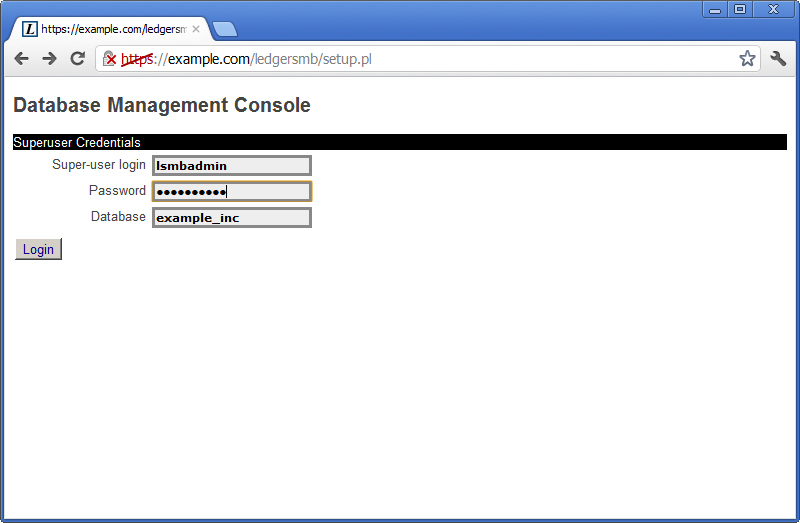
\includegraphics[width=7cm]{dmc-create-step1.png}
\caption{setup.pl login screen}
\label{fig:setup-step1}
\end{figure}

\subsection{Step 2: Company creation}

When creating a company database, there are a few things that are of importance:

\begin{itemize}
\item The name of the database is the same as the name used at login time and hence
   will be used by all users - a choice of a suitable, recognizable value is important
\item The name of the database entered (and hence the company name) is case-sensitive
\item The name can't be more than 63 characters long
% \item ### others?
\end{itemize}

After choosing ``example\_inc'' as his company name, Jack clicks the Login button at which
time the screen from \figref{fig:setup-step2} shows up. The screen says the database doesn't
yet exist and offers its creation. The backup buttons being offered are not useful at this
stage - they have value if the database exists and setup.pl is being used to upgrade
the database; one of its other functionalities.

\begin{figure}[h]
\centering
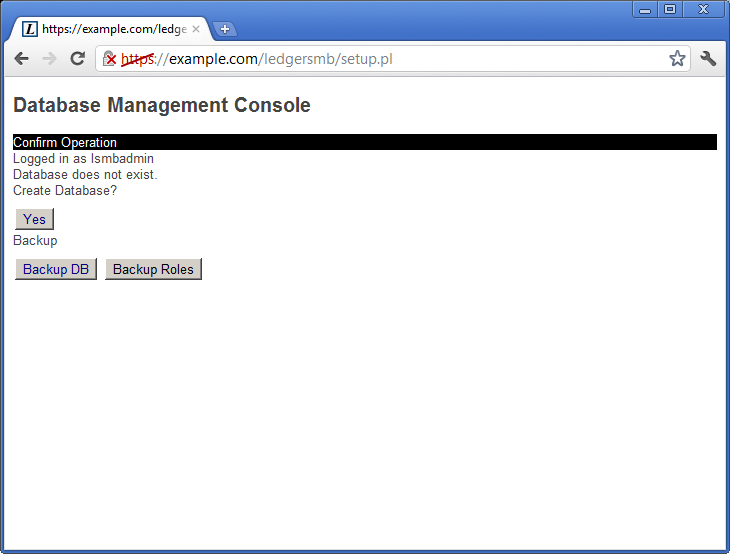
\includegraphics[width=7cm]{dmc-create-step2.png}
\caption{setup.pl company creation screen}
\label{fig:setup-step2}
\end{figure}

Jack clicks ``Yes'' to create the database and load it with LedgerSMB's database
schema, authorization rules and stored
procedures\footnote{Parts of the program inside the database.}. It may
take a while (30 seconds or more) for the next screen to appear.

\subsection{Step 3: Selection of a Chart of Accounts}

LedgerSMB comes with numerous predefined charts of accounts. These have been grouped
per country making the selection of a chart a two-step procedure. setup.pl allows for
users wanting to define their own charts by offering a ``Skip'' button. This button
skips the process of loading a chart.

\begin{quote}
Note that you need to define a chart of accounts before you can meaningfully do anything
inside LedgerSMB. If you don't load a pre-defined one you'll need to create or import your
own later.
\end{quote}

\figref{fig:setup-step3} shows the first screen in the chart of accounts selection procedure.
In this screen you select the country for which you want to use the chart of accounts. Note
that charts of accounts are highly country dependent and you may want to consult
an accountant if no default chart of accounts is included for your country.

As Jack runs his company in the US, that's what he selects.

\begin{figure}[h]
\centering
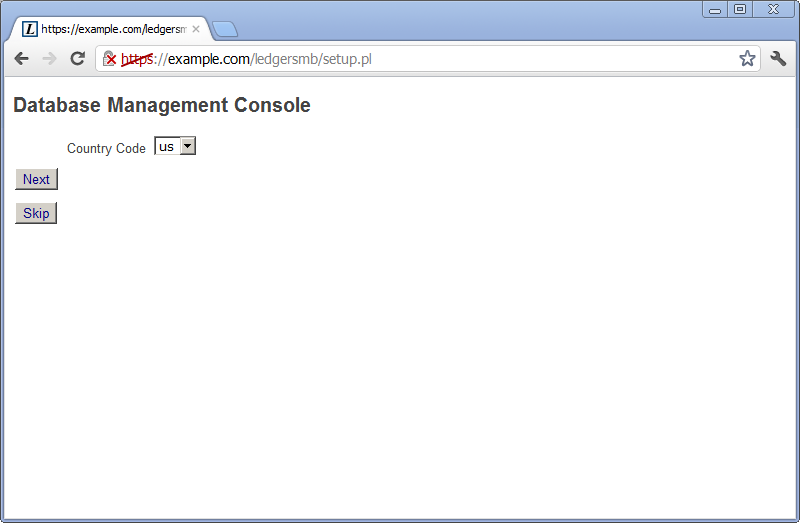
\includegraphics[width=7cm]{dmc-create-step3.png}
\caption{Chart of accounts - Country selection}
\label{fig:setup-step3}
\end{figure}

\figref{fig:setup-step4} shows the second screen in the chart of accounts selection procedure.
The drop down contains a list of all charts of accounts defined for the selected country.

Jack selects the General.sql chart of accounts: that will leave him enough room to specialize
the setup later if he has to, but for the time being offers a broadly useable setup.

\begin{figure}[h]
\centering
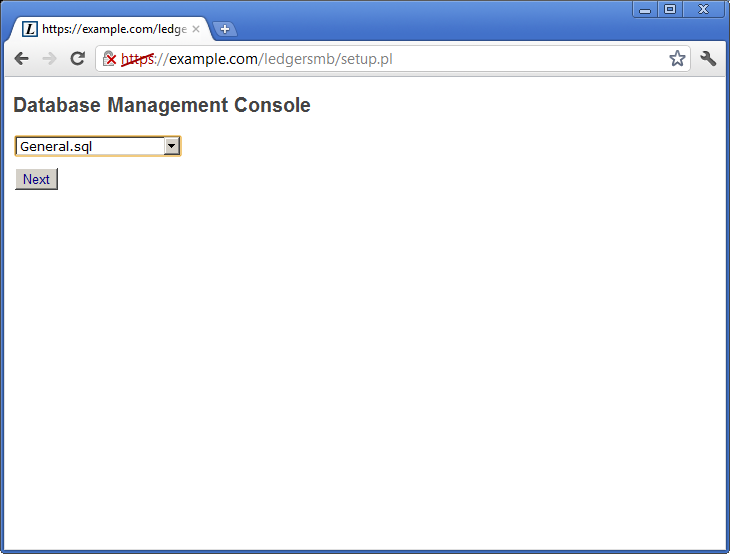
\includegraphics[width=7cm]{dmc-create-step4.png}
\caption{Chart of accounts - Chart selection}
\label{fig:setup-step4}
\end{figure}


\subsection{Step 4: First user}

In the last paragraph the technical part of the company creation procedure was completed.
However, it's not possible to log in to the company yet. This paragraph describes how to
create a first user.
\figref{fig:setup-step5} shows the user creation screen. The fields in this screen have
the same meaning as those discussed as part of user management in \secref{sec:user-creation}.

\begin{figure}[h]
\centering
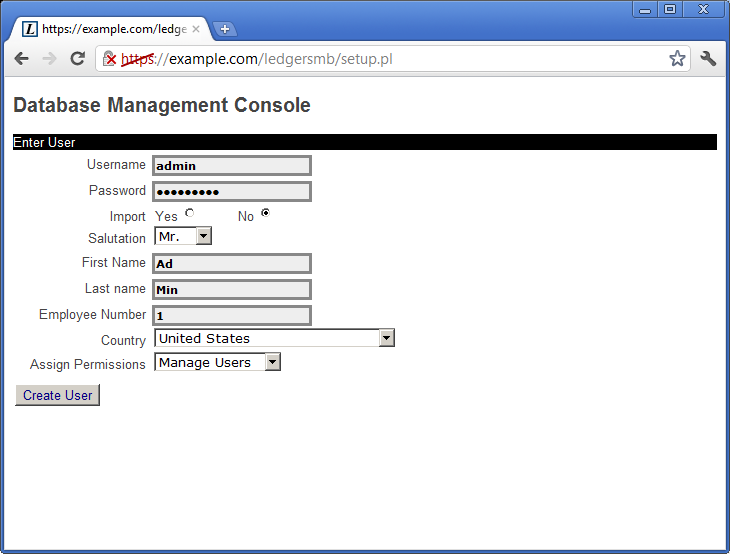
\includegraphics[width=7cm]{dmc-create-step5.png}
\caption{setup.pl initial user creation screen}
\label{fig:setup-step5}
\end{figure}

Jack chooses to create an administrative user called \texttt{admin} who will be authorized
to do everything in the application. Later on he will also create a user \texttt{jack}
who will be authorized to do everything but changing the configuration and doing application administration.
He'll use the latter user to log in for day to day operations. This will help him prevent
changing things by accident.

Note that none of the fields in this screen are optional. If the name of the user being created
isn't already used with other companies, leave the \texttt{Import} option set to \texttt{No},
otherwise please read the chapter on user creation mentioned above.

\begin{quotation}
Note: The password you enter here is a temporary one which will remain in effect for 24
hours only. Be sure to execute the steps in \secref{sec:steps-to-the-first-login} before
these 24 hours elapse, because the user will be disabled after that.
\end{quotation}

The setup.pl program offers the user to be created to be one of two types:

\begin{itemize}
\item Manage Users
\item All Permissions
\end{itemize}

Jack's choice for a fully authorized \texttt{admin} user leads him to select the
\texttt{All permissions} option.

\begin{figure}[h]
\centering
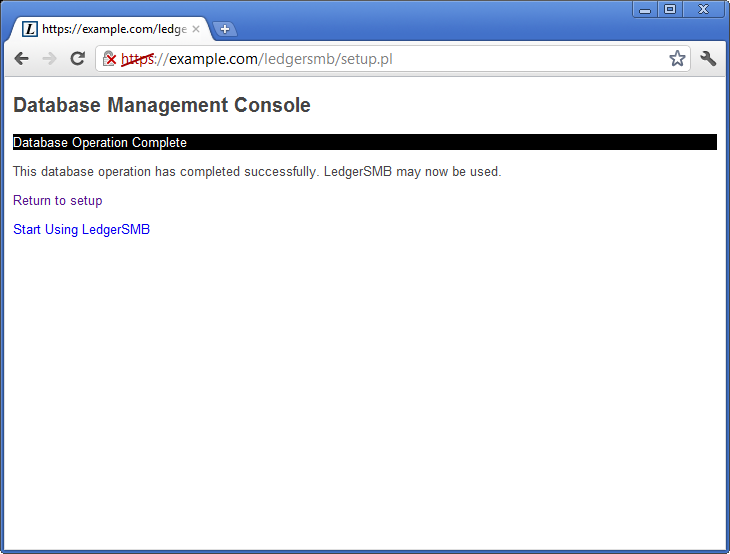
\includegraphics[width=7cm]{dmc-create-step6.png}
\caption{setup.pl successful completion screen}
\label{fig:setup-step6}
\end{figure}

Jack succeeded to correctly create his company database. His story continues in
the next chapter ``The first login''.

\section{Using create-company-database.sh}



\chapter{The first login}
\label{cha:the-first-login}

\section{Introduction}

After the company has been created by executing the procedure described in the last
chapter it is still an empty shell which needs to be populated. The correct data
needs to be entered for things like bank accounts and company contact data to be used
on invoices.

These steps have to be completed before LedgerSMB can be used meaningfully: these
settings have to be present for many workflows. A major reason is that with LedgerSMB
- as most ERP systems - financial
consequences of events in many workflows are directly reflected in the company's books.
Some accounting related settings have to be completed before LedgerSMB can do so.

This chapter documents the steps to this configuration. It assumes you've did not skip
loading a chart of accounts in \charef{cha:CompanyCreation} or that - if you did -
imported your own. Whatever your method, a chart of accounts should be available.

\section{Steps to the first login}
\label{sec:steps-to-the-first-login}

After Jack finishes the last chapter, he clicks the \texttt{Start using LedgerSMB} link
shown in \figref{fig:setup-step6}.


\subsection{Login screen}

\begin{figure}[h]
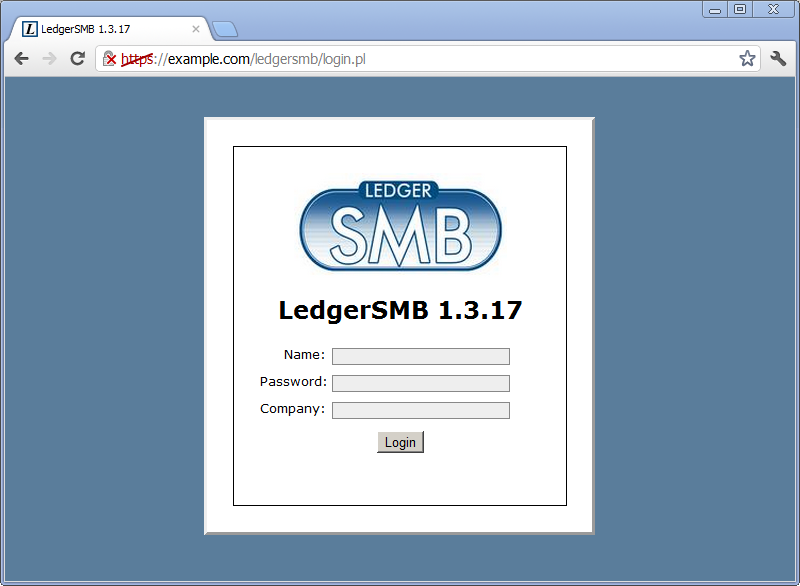
\includegraphics[width=\linewidth]{dmc-create-final.png}
\caption{login.pl opening screen}
\label{fig:login-screen}
\end{figure}

The login screen shows three fields which need to be filled out as follows:

\begin{description}
\item[Name] The user name created during database setup; Jack uses \texttt{admin}
\item[Password] The password - in this case for Jack's \texttt{admin} user
\item[Company] The name of the database created; Jack uses \texttt{example\_inc}
\end{description}

\subsection{Selecting a password}

After successful login, the system shows the user preferences screen as depicted in
\figref{fig:first-login-password} to facilitate the required password change. The
initial password has a 24-hour validity limit to prevent unused user accounts from posing
a security risk.

The password Jack chooses may be either the same as the one he used before.
Not clicking the \texttt{Save} button means the password remains unchanged and the
24-hour limit remains in effect.

\begin{figure}[h]
\centering
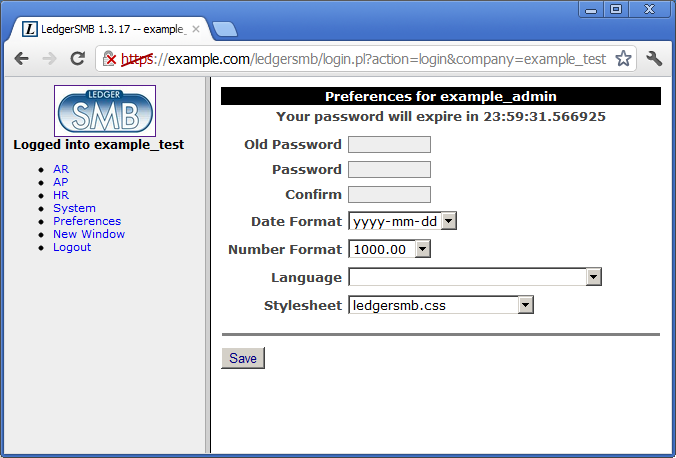
\includegraphics[width=7cm]{first-login-password.png}
\caption{First login password selection}
\label{fig:first-login-password}
\end{figure}

The new password has a validity of determined by the \texttt{Password Duration} setting
from the System $\rightarrow$ Defaults screen. User management is discussed is detail in \charef{cha:user-management}.

The password reset dialog won't show on subsequent logins until one week
before expiry. Login will be denied to users with expired passwords; they can request
password resets through user admins.


\section{Setting up the system defaults}

With the password renewal out of the way, Jack can start to set up the company for first
use. To do so, Jack selects the System $\rightarrow$ Defaults menu item.

A more elaborate description of the parameters in this screen is provided in subsection
\ref{subsec:Defaults}. However, when setting up a new company, it's probably good enough
to fill out these parameters (and thus skip the rest):

\begin{itemize}
\item Business number (e.g. Chamber of commerce number) [12345]
\item Default language [English]
\item Default accounts (Inventory, Expense, Income) [@@@]
\item Foreign exchange result accounts (Foreign exchange gain/loss) [@@@]
\item Default country [US]
\item Templates directory [demo]
\item Currencies [USD:CAD]
\item Password Duration [180]
\item Default Email From [info@example.com]
\item Company Name [Example Inc.]
\item Company Address [215 Example street - Whereitsat]
\item Company Phone [555 836 22 55]
\item Company Fax (optional) [N/A]
\end{itemize}

Jack enters the values mentioned between the square brackets in the list above. 
He used one of the charts of accounts (CoA) that came with LedgerSMB and therefore
checks the Taxes page in the System menu to see if the percentages that were delivered
with it are still current.

\section{Setting up a bank account or credit card}
\label{sec:setup-bank-account}

As part of the start up activities of his company, Jack comes to an agreement with the
bank for three products:

\begin{itemize}
\item A current account with number ``C54769''
\item Deposit account with number ``D54990''
\item Credit card with a number ending with ``.7734''
\end{itemize}

Most accounting systems - LedgerSMB included - use separate GL accounts to represent
each bank account. This allows easy reconciliation of the ending balance on the bank
account with the balance in the books.

Knowing this, Jack looks up the example bank account from his preconfigured US chart of
accounts using the System $\rightarrow$ Chart of Accounts $\rightarrow$ List Accounts menu as
shown in \figref{fig:bank-setup1}.

\begin{figure}[h]
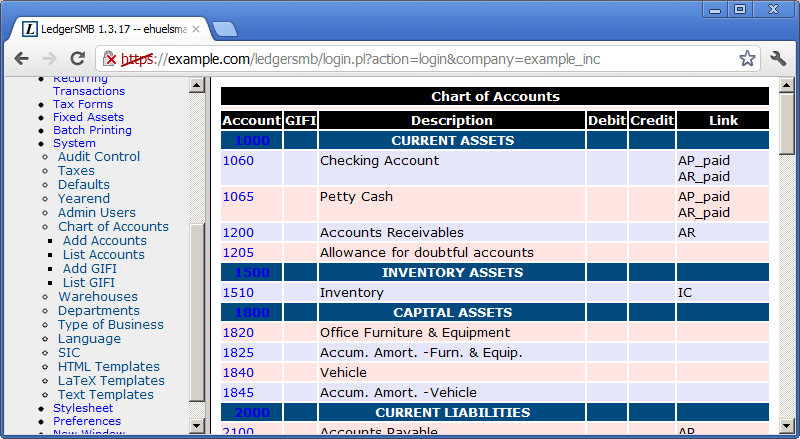
\includegraphics[width=\linewidth]{setup-bank-account1.png}
\caption{Bank account setup - menu items}
\label{fig:bank-setup1}
\end{figure}



\begin{enumerate}
\item Renames the original account 1060 ``Checking account'' into ``Checking account C54769''
\item Click ``Save''
\item Open the 1060 account again
\label{itm:bank-setup-steps-start}
\item Change the number to 1061
\item Change the description to ``Cash deposit account D54990''
\item Click ``Save as''
\label{itm:bank-setup-steps-end}
\end{enumerate}

Then Jack repeats the steps \ref{itm:bank-setup-steps-start} to \ref{itm:bank-setup-steps-end}
for the credit card with the account number 1062 and description ``Credit card xxxx.xxxx.7734'' to set
up the credit card. \figref{fig:bank-setup2} shows the screen in which to enter the account
details. \secref{sec:AccountOptions} discusses the options in detail - for now using the
settings as configured for the sample checking account will do.

\begin{figure}[h]
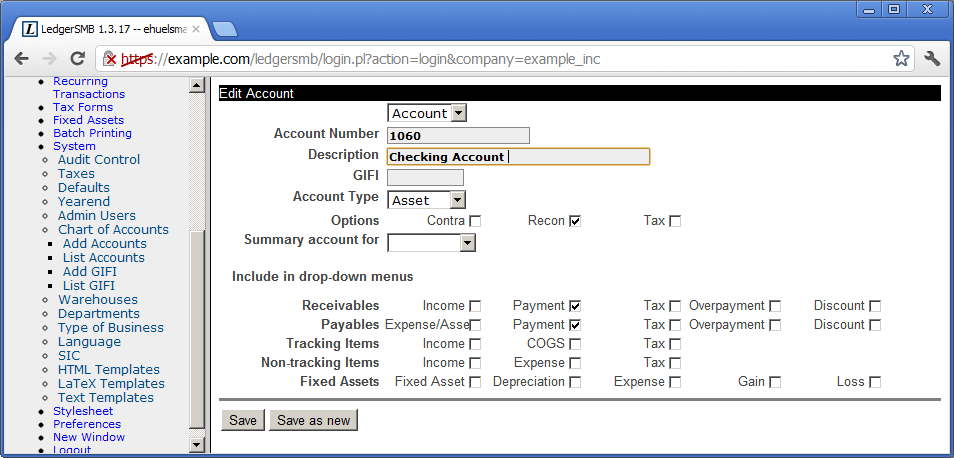
\includegraphics[width=\linewidth]{setup-bank-account2.png}
\caption{Bank account setup - account setup screen}
\label{fig:bank-setup2}
\end{figure}


\section{Checking and adjusting the chart of accounts}

Jack wants to make sure his chart of accounts fits his purposes. For now, he finds
the ledger to be in order. Although the single Sales account stands out a bit against
the numerous expense accounts, it turns out that there is also a single Purchases
account on which all the expenses for parts purchases are going to be booked.

He decides that if this isn't enough, he can add accounts later.

\section{Checking sales tax (VAT) rates}

First off, Jack asserts that a sales tax account has been provisioned. He finds it
in the Current Liabilities section of his chart of accounts. In his jurisdiction there
is only one sales tax rate applicable at any one time, which means this single account
will suit his needs just fine. If he had been in a jurisdiction with multiple tax rates
applicable, e.g. different rates for different types of goods, he would have been
required to create more accounts.

The procedure to create more sales tax accounts is the same as the one used in
\secref{sec:setup-bank-account}, with the notable difference that this time the base account
to be used is the sales tax account.

With the accounts in place, the tax rates have to be checked and possibly adjusted.
To do so, go to the System $\rightarrow$ Taxes page as shown in \figref{fig:setup-tax-rates}.

\begin{figure}[h]
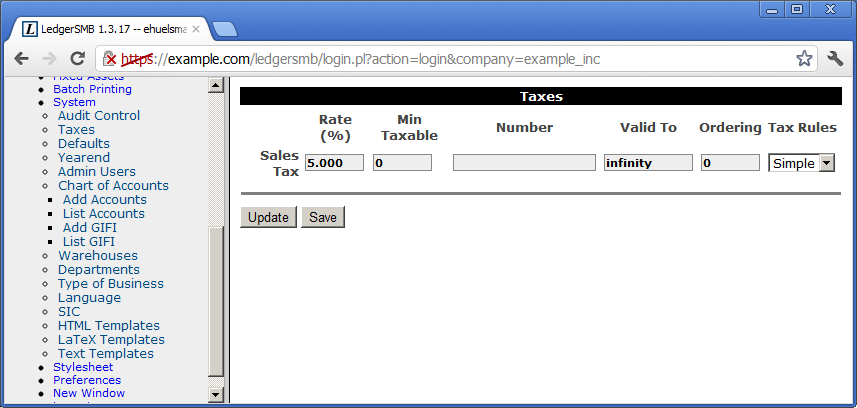
\includegraphics[width=\linewidth]{setup-tax-rates.png}
\caption{Tax rate adjustment screen}
\label{fig:setup-tax-rates}
\end{figure}

The rate shown (5\%) is exactly what Jack needs. The procedure to set rates is a bit
long to describe and hence has its own chapter. Please refer to \charef{cha:Taxes} for
details on how to change taxes.

\chapter{Building up stock}
\label{cha:building-up-stock}

\chapter{Ramping up to the first sale}
\label{cha:ramping-up-to-the-first-sale}

% sending out a quote followed by a sales order

\chapter{Shipping sales}
\label{cha:shipping-sales}

\chapter{Invoicing}
\label{cha:invoicing}

\section{Handling sales taxes}

% invoices with taxes included

% invoices with explicit tax amounts

% 


\chapter{Collecting sales invoice payments}
\label{cha:customer-payments}

\section{Customer payments}

\section{Customer payment mismatch}

% choosing between pardonning and registering underpayment

% large ones, as in partial payments or largish under/over payments

% pardonning small mismatches


\chapter{Paying vendor invoices}
\label{cha:vendor-payments}

% handling vendors who match amounts to exact invoices

% handling vendors with running balances

% handling bounced checks: voiding checks to undo payments of vendor invoices
%   relating to bounced checks

\chapter{Monitoring arrears}
\label{cha:monitoring-arrears}

% handling interest on arrears

\chapter{Branching out: services}

% including creation / assignment to different accounts


\section{Recording service hours}

\section{Customer approval on service hours}

\section{Invoicing services}

\chapter{Branching out II: service subscriptions}


